\section{第二问：化合物关联结构与关键因素}\label{sec:q2}

\subsection{共表达图的构建}

高相关只集中在少数化合物族，多数字段与其他字段近似独立，图正则能够影响的系数范围因此在建模之前就已受限。在 250 款酒的全部 231 个数值字段上计算 Spearman 秩相关，保留 $|r|\ge0.7$ 的字段对作为边，边权取带符号的相关系数，得到 231 个节点、109 条边。浓度字段跨越多个数量级且含截尾值，秩相关对单调变换不敏感，适合这种分布。有边的字段只有 81 个，其余 150 个字段没有任何邻居，约占全部字段的三分之二。

81 个非孤立字段被划为 19 个模块，最大模块含 15 个字段，109 条边的平均 $|r|$ 为 0.79，模块成员与化合物族基本对应。最大的两块以脂肪酸乙酯、乙酸酯和发酵综合量为主，包括乙酸乙酯、辛酸乙酯、癸酸乙酯、乙酸苯乙酯、乙醇、甘油与酯类总量；随后是酒花倍半萜烯氧化物（石竹烯氧化物、蛇麻烯环氧化物 II、$\alpha$-木罗醇等）、C$_6$—C$_9$ 高级醇（3-甲基-2-己醇、1-辛醇、4-甲基-1-戊醇等）与单萜醇（linalool、$\alpha$-松油醇、香茅醇）。酯类主要来自酵母的酯合成，酒花萜烯随酒花添加进入，高级醇是发酵副产物，模块因此沿原料与代谢途径分层；同类化合物共享前体与合成途径，这是高相关只出现在少数族内的化学原因。

109 条边全部为正相关，最小 $r$ 为 0.703，本数据中没有出现 $|r|\ge0.7$ 的负相关字段对。有符号权重保留了方法的一般性，但“负相关边鼓励系数反向”的机制未被触发，后文的图惩罚实际只做同向平滑。

图\ref{fig:net}(a) 把邻接矩阵按模块排序，非零元集中在少数对角块内，块外接近空白；图\ref{fig:net}(b) 给出模块规模，除前几个模块外，其余模块只含 2—3 个字段。同类化合物由同一原料或同一代谢途径产生，因而同向共变，这与以化合物谱预测复杂风味的既有结果一致\cite{schreurs2024}。孤立字段并非无关紧要，它们只是缺少 $|r|\ge0.7$ 的强共变伙伴，其系数只能由自身与目标的关系决定；孤立字段的拉普拉斯行恒为零，图惩罚只能在 81 个字段内部传递信息。

以上网络在全部数据上估计，用于描述。

阈值决定图的疏密。把 $|r|$ 的门槛由 0.6 提到 0.9，边数从 266 条降到 9 条，非孤立字段从 130 个降到 15 个（表\ref{tab:threshold}）。0.7 是折中：再低会把经由第三变量产生的间接关联连进来，模块结构被稀释；再高只剩 9 条边，94\% 的字段成为孤立点，图惩罚几乎无处可施。0.7用于全数据网络的描述；模型验证时在每个训练折重算相关图，并在内层候选阈值0.6、0.7、0.8中选参。

\begin{table}[t]
\centering\small\renewcommand{\arraystretch}{1.15}
\caption{相关阈值对网络结构的影响（231 个字段）}
\label{tab:threshold}
\begin{tabular}{@{}cccc@{}}
\toprule
阈值 $|r|$ & 边数 & 连通分量 & 孤立字段 \\
\midrule
0.6 & 266 & 114 & 101 \\
0.7 & 109 & 169 & 150 \\
0.8 & 39  & 207 & 194 \\
0.9 & 9   & 222 & 216 \\
\bottomrule
\end{tabular}
\end{table}
建模时相关图在每个训练折内单独重算，测试折不参与，图结构与评价样本保持分离。

\begin{figure*}[t]
\centering
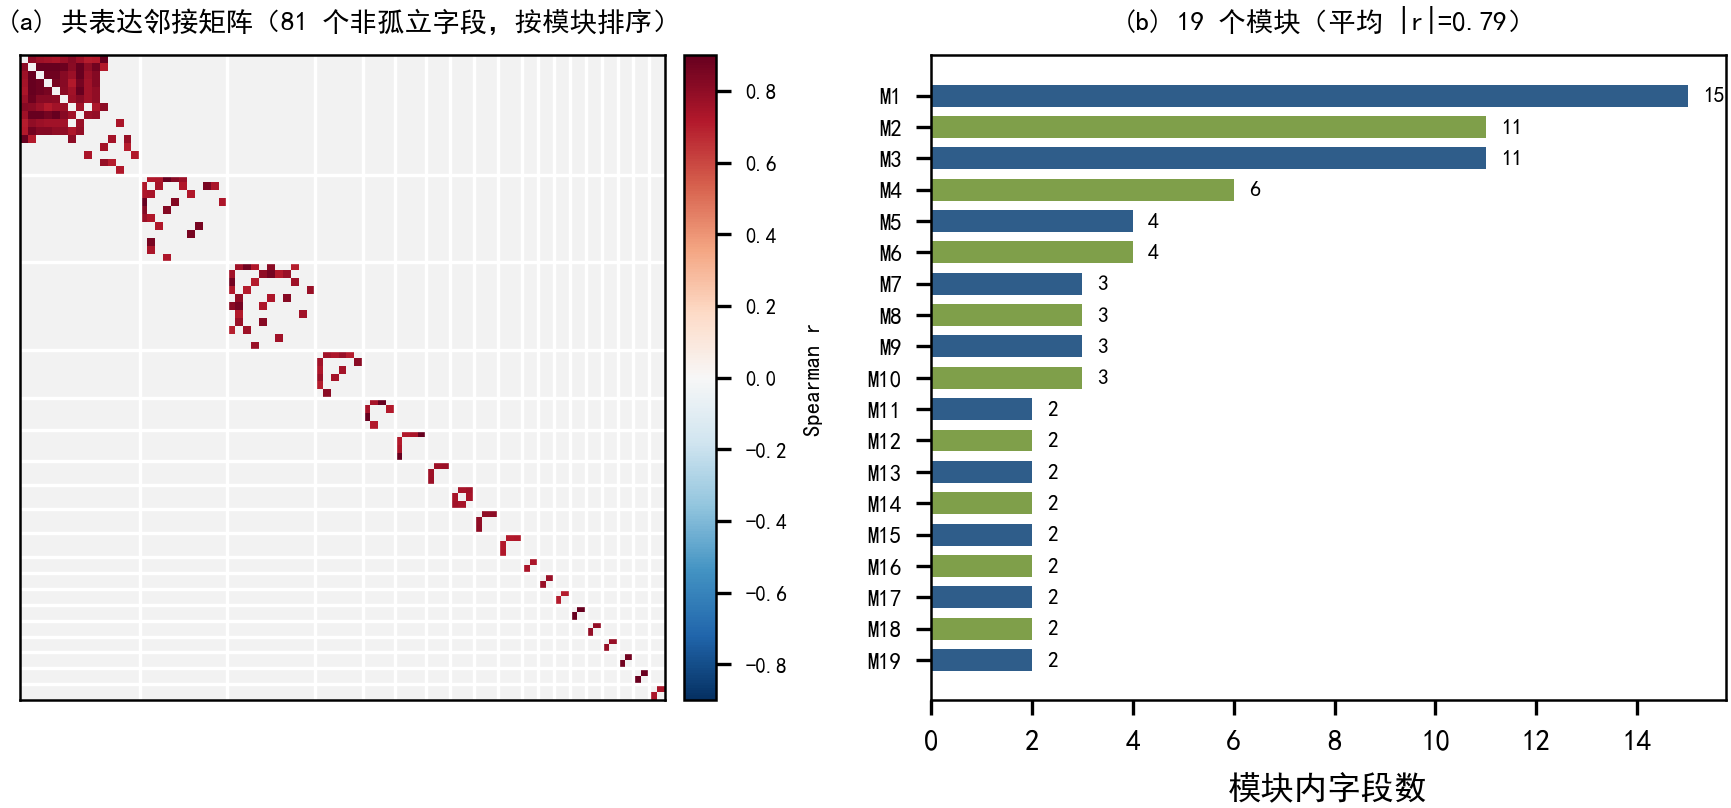
\includegraphics[width=0.98\textwidth]{figures/fig09_network.png}
\caption{共表达网络的结构。(a) 81 个非孤立字段的邻接矩阵按模块排序，非零元集中于少数对角块，块外基本空白；(b) 19 个模块的规模，除前几个模块外均只含 2—3 个字段。}
\label{fig:net}
\end{figure*}

\subsection{图约束模型与可解性}

图约束模型在 $\alpha>0$、$\lambda\ge0$ 时严格凸、解唯一，三种图设定之间的误差差异因此来自惩罚项中的图结构，而不是求解过程。

记标准化后的化合物矩阵为 $Z\in\mathbb{R}^{250\times231}$，中心化后的感官均分矩阵为 $Y_c\in\mathbb{R}^{250\times50}$，待估系数矩阵为 $B\in\mathbb{R}^{231\times50}$。图用带符号权重矩阵 $W$ 表示，拉普拉斯矩阵取 $L=\operatorname{diag}(\sum_j|W_{ij}|)-W$，模型为

\begin{equation}
\begin{aligned}
\hat{B}=\arg\min_{B}\Bigl\{&\|Y_c-ZB\|_F^2+\alpha\|B\|_F^2\\
&+\lambda\operatorname{tr}(B^{T}LB)\Bigr\}.
\end{aligned}
\label{eq:graph}
\end{equation}

式\eqref{eq:graph} 的第一项是拟合误差，第二项是岭惩罚，第三项让正相关邻边的系数接近、负相关邻边的系数方向相反；$\lambda=0$ 时模型退化为普通岭回归。$\lambda$ 增大时，系数更受带符号邻边的约束；若负边构成符号不平衡的环，图惩罚的零空间不必保留每个分量的一个自由度。$\alpha$ 控制整体收缩的强度，$\lambda$ 控制沿边差异的强度，两者共同决定模型的有效自由度，这也是二者需要在折内同时选择的原因。

对任一系数向量 $b$，有

\begin{equation}
b^{T}Lb=\sum_{i<j}|W_{ij}|\left(b_i-\operatorname{sign}(W_{ij})b_j\right)^2\ge0.
\label{eq:psd}
\end{equation}

式\eqref{eq:psd} 可由 $b^{T}Lb=\sum_i\sum_j|W_{ij}|b_i^2-2\sum_{i<j}W_{ij}b_ib_j$ 逐项配方得到。右边每个平方项非负，故 $L$ 半正定；等号成立当且仅当在 $W$ 的每个连通分量内 $b_i=\operatorname{sign}(W_{ij})b_j$，即系数沿边的符号保持一致。

由式\eqref{eq:psd}，$\lambda$ 项是 $B$ 的凸函数；$\alpha>0$ 使 $\alpha\|B\|_F^2$ 的 Hessian 为 $2\alpha I$，目标函数强凸，式\eqref{eq:graph} 因而有唯一解。等价地，正规方程 $(Z^{T}Z+\alpha I+\lambda L)B=Z^{T}Y_c$ 的系数矩阵正定。若 $\alpha=0$，带符号 $L$ 的零空间由各边的符号约束决定，唯一性取决于 $Z$ 与 $L$ 的共同零空间；本文字段存在强共线，正岭惩罚因此不可省去。50 个目标共享同一个 $L$，惩罚不跨目标耦合，每个目标等价于一个单独的正则回归；图只改变同一目标内部不同字段的系数分配，不改变目标之间的相对难度。

参数与外层评价严格分离：$\alpha$、$\lambda$ 与相关阈值都在每个训练折内部由内层留出误差选择，外层测试折不参与；同一折内另取 10 个节点标签随机置换的图，按相同流程重建并重新选参，作为结构无关的零模型。零模型也经过调参，误差中包含选择波动，比较时按同一协议解读。图结构回归的惩罚形式取自图结构变量的回归与选择\cite{li2010}。

\subsection{双口径结果}

真实图的差值随评价口径变号：单折口径比无图差0.000124分，五次预测聚合后好0.001283分。结合效应量和最终全数据选参，现有证据不支持图正则具有稳定且实际意义明确的预测优势；网络主要用于描述化学共变结构。

两种口径评价不同对象。单折口径把 15 个外层折的留出 MAE 再平均，每次拟合只产生一次预测，对应“训练一次即上线”的误差；聚合口径先对同一款酒的五次留出预测取平均，再在 250 款酒上计算 MAE，对应“重复建模、预测取均值”的误差。前者的样本单位是折，后者是酒；前者保留单次拟合的方差，后者通过平均削去一部分方差。同一批预测在两种口径下给出相反符号，说明图的效应与汇总方式有关，不能脱离口径单独陈述；两种口径对应不同的部署假设，并列报告才能覆盖两种使用场景。

表\ref{tab:graph} 给出核心 30 项的结果。单折平均为无图 0.536911、真实图 0.537035、打乱图 0.537794；聚合预测为无图 0.526148、真实图 0.524865，差值 $-0.001283$，固定预测条件下以酒为单位重采样2000次的 95\% 区间为 $[-0.002341,-0.000229]$。该区间以固定留出预测为条件，不包含重训与选参的不确定性；区间未跨0，但误差差值仅0.001283分，实际意义需要结合任务精度判断。

\begin{table*}[t]
\centering\small\renewcommand{\arraystretch}{1.2}
\caption{核心 30 项在图模型三种设定下的 MAE}
\label{tab:graph}
\begin{tabular}{@{}lcccc@{}}
\toprule
评价口径 & 无图 & 真实图 & 打乱图 & 真实图减无图 \\
\midrule
单折平均（15 个外层折） & 0.536911 & 0.537035 & 0.537794 & $+0.000124$ \\
聚合预测（按酒平均） & 0.526148 & 0.524865 & — & $-0.001283$ \\
\bottomrule
\end{tabular}
\end{table*}

打乱图作为结构对照，在单折口径下平均误差最高；该结果本身不能分离随机图平滑和选参造成的差异。真实图与无图的差距很小。效应小有结构性原因：150 个字段是孤立节点，其系数行不受图惩罚；15 个外层折中只有 7 折选到正的 $\lambda$，其余 8 折的 $\lambda=0$，模型退化为岭回归。图只在不到一半的折里对 81 个字段中的一部分起作用，最优强度在多数折内被内层准则判为零。

聚合口径把每款酒的五次预测平均。重复划分的训练集相互重叠，五次预测存在相关性，平均后的方差不能假定缩减至五分之一；本实验没有分解图惩罚对偏差与方差的影响。

全 50 项的单折结果为无图 0.470061、真实图 0.470220、打乱图 0.471037，排序与核心 30 项一致，差异同样在万分位。 最终描述模型由全部数据上的三折内层验证按核心30项MAE选择参数，重算网格中 $\alpha=1000,\lambda=0$ 的内层误差为0.539083；最佳正图惩罚组合为 $\alpha=1000,\lambda=1,\tau=0.8$，误差为0.539086。选参依据是内层误差和既定网格排序，不是使用外层聚合误差或重采样区间直接选取 $\lambda$。最终用全部数据拟合的描述模型选得 $\lambda=0$，Top-3 由岭回归系数给出。图在本文中承担解释功能，不是预测模型的组成部分；把它写成“提升了预测精度”会与最终选择矛盾。

\subsection{Top-3 的稳定性}

150 条候选中只有 36 条同时满足频率、折数与置换贡献三项条件；Top-3 对单元格级异常稳健，对变量集合敏感，因此不能读作变量选择结论。

对 50 个目标各取标准化岭回归系数绝对值最大的 3 个字段，共 150 条记录。以酒为单位做 200 次 bootstrap，同一款酒的各目标一起进出，目标间的相关性不被打破；每次重建预处理与相关图，并固定全数据选定的 $\alpha$、$\lambda$ 与阈值，记录字段是否仍在该目标的前三位，得到入选频率\cite{efron1993}；同时统计 15 个外层折中的入选次数，以及留出数据上普通置换与风格内置换的误差增量。支持条件为频率不低于 0.5、至少在 5 个外层折入选、两种置换的平均贡献均为正，三项分别对应重采样稳定性、跨折稳定性与预测贡献。

单看频率有 46 条不低于 0.5，且都至少在 5 折入选；再要求两种置换贡献为正，剩 36 条，被剔除的 10 条都是置换贡献不稳定的记录。36 条候选分布在 29 个目标上：22 个目标各 1 条、7 个目标各 2 条，其余 21 个目标没有任何候选通过。图\ref{fig:top3}(a) 给出 150 条候选的入选频率分布，0.5 的门槛把候选分成通过与否两组，0.2—0.4 区间仍聚集了相当一部分记录，这些字段只是偶尔进入前三；图\ref{fig:top3}(b) 按目标给出通过比例，空白目标即没有候选通过。频率以固定参数为条件；若在每次重采样中重新选参，评估的是完整选择流程的稳定性。0.5 是本文采用的描述性门槛，不是显著性水平，门槛附近的频率差别不宜过度解读。

\begin{figure*}[t]
\centering
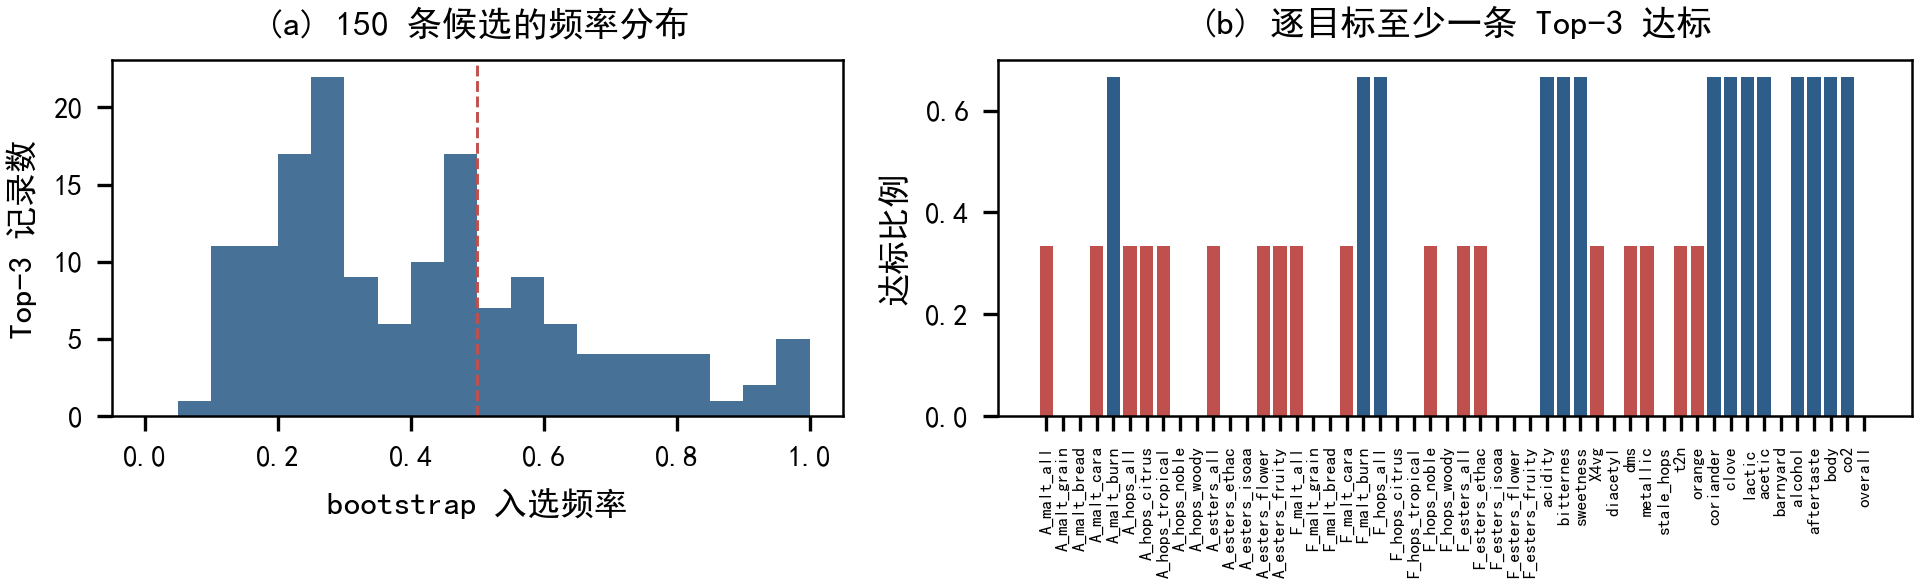
\includegraphics[width=0.98\textwidth]{figures/fig10_top3.png}
\caption{Top-3 的稳定性。(a) 150 条候选的 bootstrap 入选频率分布，虚线为 0.5 的门槛；(b) 逐目标通过支持条件的候选比例，空白目标表示没有候选通过。}
\label{fig:top3}
\end{figure*}

化学异常敏感性见表\ref{tab:top3}。把 80 个异常单元格置为缺失、仅用训练折估计填补后，核心 30 项 MAE 由 0.50641 变为 0.50691，全 50 项由 0.44478 变为 0.44515，预测值平均绝对变化 0.00500 分，Top-3 平均保留 97.64\%。仅使用第\ref{sec:scale}节所定义的 $V$（38个逐点一致字段、61个单位登记字段及226个非综合字段的交集）时，固定 $\alpha=1000$ 的15折岭回归 Top-3 平均保留36.18\%。该 $V$ 与含80处异常的32个字段完全不同，交集为空。

\begin{table*}[t]
\centering\small\renewcommand{\arraystretch}{1.2}
\caption{Top-3 的支持条件与化学异常敏感性}
\label{tab:top3}
\begin{tabular}{@{}lcc@{}}
\toprule
检验项目 & 数值 & 备注 \\
\midrule
通过支持条件的记录 & 36 / 150 & 频率$\ge0.5$、$\ge5$ 折入选、置换贡献为正 \\
核心 30 项 MAE（异常置缺失前 $\to$ 后） & 0.50641 $\to$ 0.50691 & 分 \\
全 50 项 MAE（异常置缺失前 $\to$ 后） & 0.44478 $\to$ 0.44515 & 分 \\
预测值平均绝对变化 & 0.00500 & 分 \\
Top-3 平均保留（异常置缺失） & 97.64\% & — \\
Top-3 平均保留（仅交集 $V$ 的32字段） & 36.18\% & — \\
\bottomrule
\end{tabular}
\end{table*}

两类扰动都改变输入，性质不同。前者只抹掉 80 个单元格，受影响字段仍由其余酒样支撑，系数排序几乎不动；后者把226个非综合字段压到交集 $V$ 的32个字段，候选池本身换掉，Top-3 只剩约三分之一。稳定的 Top-3 是“在当前字段集合与当前模型下稳定”，不是变量选择结论；换一套输入，排名会重排。

\subsection{化学解释及其边界}

三个例子分属三种证据强度：同名端点上的近确定性关联、机制清楚但经由未观测过程的关联、文献支持而统计支持不足的关联。系数、相关与入选频率都是关联量，单独任何一项都不构成因果证据。

X4VG 与 X4vg 的关系最强。X4VG 在该端点上的入选频率为 1.00，15 个外层折全部入选，系数为正。4VG 是阿魏酸经酵母脱羧的产物，赋予丁香与酚类香气，储藏中会下降并转化为香草醛等物质\cite{vanbeneden2008}。这一条的证据链最完整，但端点本身以该化合物命名，关联接近定义对应，属于模型复现命名关系，而不是独立发现。

iron 与 metallic 的关系次之。iron 在 metallic 上的入选频率为 0.94，15 个外层折全部入选，系数为正。铁不是香气化合物，金属感来自口腔中脂质氧化与铁离子的催化过程\cite{omur2012}；模型看到的是铁含量高的酒更容易被评出金属感这一共变，催化链本身没有进入模型。铁还与水质、设备与风格相关，当前设计无法把铁从这些过程变量中分离。iron 同时进入酒花香气、苦味与甜味等性质不同的端点，这种跨端点重复更像风格或工艺的代理变量，而不是某一感官属性的专属因素。

linalool 与 coriander 的关系最弱。linalool 以 0.46 的频率列第三，低于 0.5 的门槛，只在 8 个外层折入选。芫荽籽是小麦啤酒的传统香料，其添加阶段与用量会改变啤酒中的 linalool 含量\cite{pater2024}，文献给出的来源关系与正系数方向相容，但统计支持没有过线。文献支持与重采样稳定性是两个独立维度，前者不能替代后者。置换贡献衡量字段取值对留出误差的作用，贡献为正只说明该字段携带预测信息，不说明它通过化学途径影响感官。

共线化合物会在系数上互相替代。同一模块内的字段通过 $|r|\ge0.7$ 的边直接或间接相连，相关变量可能在系数排序中相互替代；模块级联合置换结果提供补充证据，但不能预设所有模块的系数和都稳定。可信的解释应落在模块层面，例如酒花倍半萜烯氧化物或脂肪酸乙酯这样的族，单个化合物名称只作为该族的代表。按模块报告时，“该族整体为正”与“族内某个化合物排名靠前”需要分开陈述，前者对共线替代不敏感。附件 8 的 GBM SHAP 与 MDI 来自原始研究的模型，本文只将其作为外部参照核对化学方向，不计入本队结果\cite{lundberg2017}。可检验的解释顺序是：先看模块是否与原料或工艺对应，再看代表化合物的方向与文献是否一致，最后用独立批次验证。
